\chapter{Results}
This chapter discusses the results we obtained by processing data on HCP pipelines. The differences we observed and the quantified metric values are discussed in detail for each pipeline. Section \ref{sec:Prefreesurfer} discusses PrefreeSurfer results, followed by section \ref{sec:Freesurfer} on FreeSurfer results, section \ref{sec:Postfreesurfer} on PostFreeSurfer results and last section \ref{sec:fMRI} discusses fMRIVolume pipeline results.

\section{PreFreeSurfer} \label{sec:Prefreesurfer}
I analyzed the subjects processed on CentOS6 and CentOS7 using the PreFreeSurfer pipeline. The differences found in files due to the processing on two different operating systemis described in this section.

\subsection{Inter-OS differences}
Among the 92 NIFTI imaging files common to all 5 subjects, 76 (.nii.gz) files differed between CentOS6 and CentOS7. Figure~\ref{fig:prefreesurfer_metric_values} shows the Dice coefficient value and NRMSE values of the nifti files that were found to have differences in between operating systems. The mean, median and standard deviation NRMSE and Dice coefficien values are given in Table~\ref{tab:PreFreeSurfer_Metic_Values}.
\hfill \break
\begin{center}
\begin{tabular}{|l|l|l|}
\hline
Item               & NRMSE       & DICE        \\ \hline
Mean               & 0.006998923 & 0.229517835 \\ \hline
Median             & 0.003744135 & 0.02166149  \\ \hline
Standard Deviation & 0.013993721 & 0.337104803 \\ \hline
\end{tabular}
\captionof{table}{NRMSE \& DICE values for PreFreeSurfer processing on CentOS6 and CentOS7}
\label{tab:PreFreeSurfer_Metic_Values}
\end{center}
\hfill \break
The below list of files  are consistently different across the subjects (Std. Deviation (NRMSE) $\leq$ .003).
\begin{itemize} 
  \item T2w/T2wToT1wDistortionCorrectAndReg/FieldMap2T1w\_acpc\_ShiftMap.nii.gz
  \item T1w/BiasFieldCorrection\_sqrtT1wXT1w/bias\_raw.nii.gz
  \item T2w/BrainExtraction\_FNIRTbased/NonlinearReg.nii.gz
  \item T2w/BrainExtraction\_FNIRTbased/NonlinearIntensities.nii.gz
  \item T2w/T2wToT1wDistortionCorrectAndReg/T2w2T1w/sqrtT1wbyT2w.nii.gz
\end{itemize}

Files with NRMSE value that vary specifically for each subject are listed below (Std. Deviation $\geq$ 0.15).
\begin{itemize}
  \item T1w/BiasFieldCorrection\_sqrtT1wXT1w/T1wmulT2w.nii.gz
  \item MNINonLinear/xfms/NonlinearIntensities.nii.gz
  \item T2w/BrainExtraction\_FNIRTbased/NonlinearRegJacobians.nii.gz
  \item T1w/BrainExtraction\_FNIRTbased/standard2str.nii.gz
  \item T2w/T2wToT1wDistortionCorrectAndReg/T2w2T1w/T2w\_dc\_reg.nii.gz
\end{itemize}

Files that got a zero value (zero similarity) for the Dice coefficient are listed below,
\begin{itemize}
\item T1w/T1w\_acp\c\_dc.nii.gz
\item T1w/ACPCAlignment/acpc\_final.nii.gz
\item T2w/T2w.nii.gz
\end{itemize}

Files with Dice coefficient that vary specifically for each subject is listed below (Std. Deviation $\geq$ .18),
\begin{itemize}
\item T1w/BiasFieldCorrection\_sqrtT1wXT1w/T1wmulT2w.nii.gz
\item T2w/BrainExtraction\_FNIRTbased/NonlinearIntensities.nii.gz
\item T2w/BrainExtraction\_FNIRTbased/NonlinearRegJacobians.nii.gz
\item MNINonLinear/xfms/NonlinearIntensities.nii.gz
\end{itemize}

\begin{center}
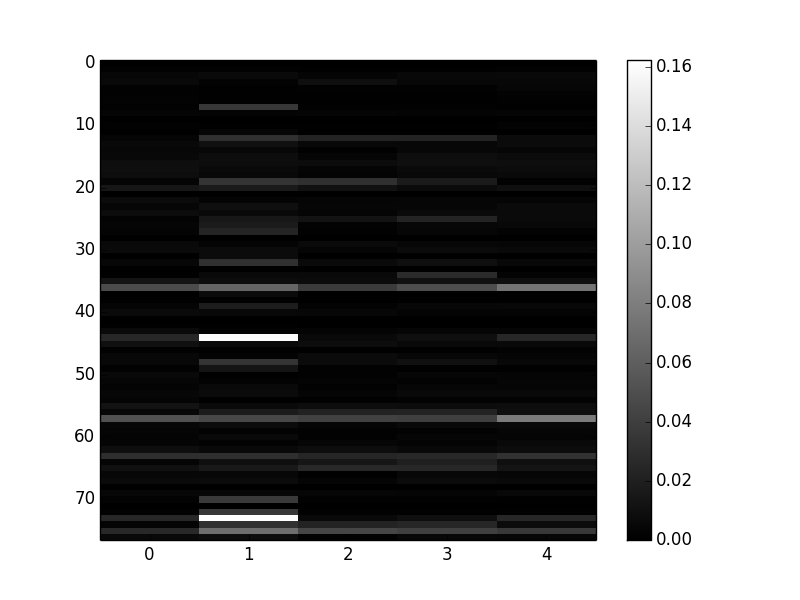
\includegraphics[width=.5\linewidth]{prefreesurfer_nrmse.png}%
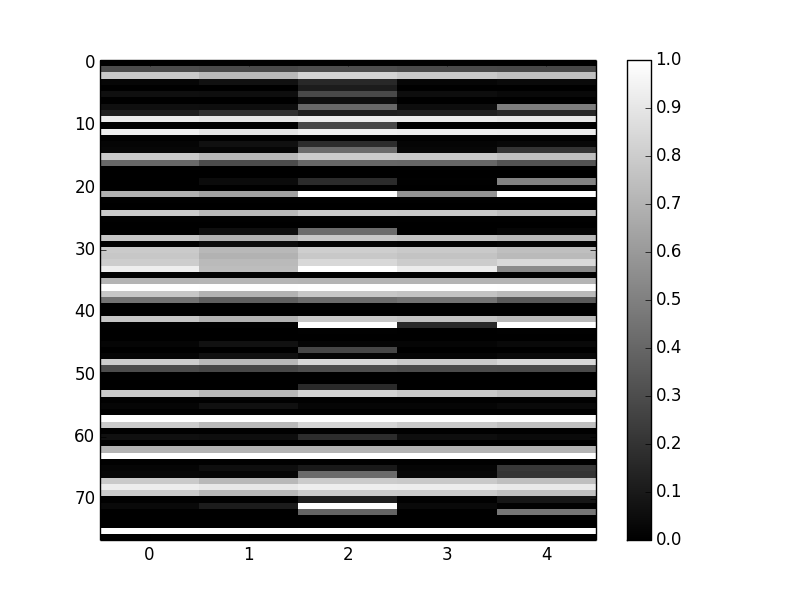
\includegraphics[width=.5\linewidth]{prefreesurfer_dice.png}
\captionof{figure}{PreFreeSurfer metric values}
\caption*{(i) NRMSE (left) (ii)Dice coefficient (right)}
\label{fig:prefreesurfer_metric_values}
\end{center}

\section{FreeSurfer} \label{sec:Freesurfer}
FreeSurfer results presented in this section does not take into account the files that were found to be different in PreFreeSurfer pipeline. The number of files that has differences and which are common to all the subjects, was found to be 61 files (23 .nii.gz files and 38 .mgz files). Table~\ref{tab:FreeSurfer_Metic_Values} gives the details about the mean, median and standard deviation of NRMSE and Dice coefficient values. Figure~\ref{fig:freesurfer_metric_values} illustrates the NRMSE and Dice coefficient values in the form of mat
\hfill \break
\begin{center}
\begin{tabular}{|l|l|l|}
\hline
Item               & NRMSE       & DICE        \\ \hline
Mean               & 0.017669782 & 0.695379753 \\ \hline
Median             & 0.009735296 & 0.926226795 \\ \hline
Standard Deviation & 0.018183193 & 0.405144714 \\ \hline
\end{tabular}
\captionof{table}{NRMSE \& DICE values for FreeSurfer processing on CentOS6 and CentOS7}
\label{tab:FreeSurfer_Metic_Values}
\end{center}
\hfill \break
The files listed below are consistently different across the subjects with respect to the NRMSE value (Std. Deviation $\leq$ .00003).
\begin{itemize}
\item T1w/subject\_name/mri/T1w\_hires.greynorm.nii.gz
\item T1w/subject\_name/mri/T1w\_hires.greynorm.mgz
\item T1w/subject\_name/mri/ribbon.postT2.pass1/T1w\_hires.greynorm\_ribbon.nii.gz
\end{itemize}

Files with NRMSE value that vary specifically for each subject are listed below (Std. Deviation $\geq$ 0.008).
\begin{itemize}
\item T1w/subject\_name/mri/ribbon.postT2.pass1/rh.ribbon.nii.gz
\item T1w/subject\_name/mri/ribbon.postT2.pass1/ribbon.nii.gz
\item T1w/subject\_name/mri/ribbon.postT2.pass1/ribbon\_inv.nii.gz
\end{itemize}

Files that are consistently different across subjects are listed below with respect to the Dice coefficient are listed below (Std. Deviation $\leq$ .000001).
\begin{itemize}
  \item T1w/subject\_name/mri/T2w\_hires.norm.nii.gz
  \item T1w/subject\_name/mri/T2w\_hires.norm.mgz
  \item T1w/T1w\_acpc\_dc\_restore\_1mm.nii.gz
  \item T1w/subject\_name/mri/rawavg.mgz
  \item T1w/subject\_name/mri/orig/001.mgz
\end{itemize}

Files with Dice coefficient that vary specifically for each subject is listed below (Std. Deviation $\geq$ .055).
\begin{itemize}
\item T1w/subject\_name/mri/ribbon.postT2.pass1/ribbon\_s5.nii.gz
\item T1w/subject\_name/mri/transforms/talairach.m3z.inv.y.mgz
\item T1w/subject\_name/mri/transforms/talairach.m3z.inv.x.mgz
\item T1w/subject\_name/mri/transforms/talairach.m3z.inv.z.mgz
\end{itemize}
\hfill \break
\begin{center}
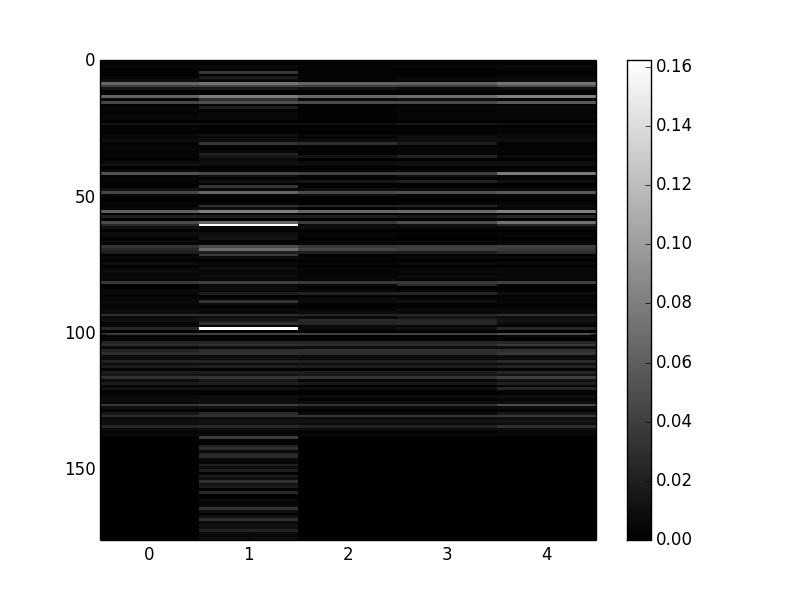
\includegraphics[width=.5\linewidth]{freesurfer-nrmse.png}%
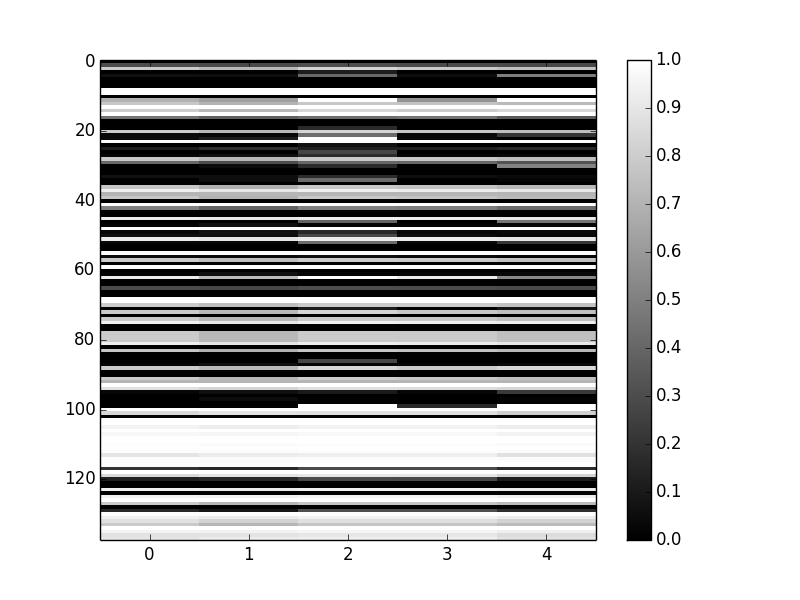
\includegraphics[width=.5\linewidth]{freesurfer-dice.png}
\captionof{figure}{FreeSurfer metric values}
\caption*{(i) NRMSE (left) (ii)Dice Coefficient (right)}
\label{fig:freesurfer_metric_values}
\end{center}

\section{PostFreeSurfer}\label{sec:Postfreesurfer}
25 (.nii.gz) files that were common to all the subjects and which were produced as part of PostFreeSurfer processing was found to have differences. Table~\ref{tab:PostFreeSurfer_Metic_Values} contains the mean, median and standard deviation values we obtained from these 25 files across the subjects. 
\hfill \break
\begin{center}
\begin{tabular}{|l|l|l|}
\hline
Item               & NRMSE       & DICE        \\ \hline
Mean               & 0.03474272  & 0.676874536 \\ \hline
Median             & 0.038619041 & 0.982912774 \\ \hline
Standard Deviation & 0.025485142 & 0.458426209 \\ \hline
\end{tabular}
\captionof{table}{NRMSE \& DICE values for PostFreeSurfer processing on CentOS6 and CentOS7}
\label{tab:PostFreeSurfer_Metic_Values}
\end{center}
\hfill \break

The files listed below are consistently different across the subjects with respect to the NRMSE value (Std. Deviation $\leq$ .0004).
\begin{itemize}
  \item MNINonLinear/ROIs/Atlas\_wmparc.2.nii.gz
  \item T1w/xfms/OrigT1w2standard.nii.gz
  \item T1w/xfms/OrigT2w2standard.nii.gz
  \item T1w/xfms/OrigT1w2T1w.nii.gz
  \item T1w/xfms/OrigT2w2T1w.nii.gz
\end{itemize}

Files with NRMSE value that vary specifically for each subject are listed below (Std. Deviation $\geq$ 0.007).
\begin{itemize}
  \item T1w/aparc.a2009s+aseg.nii.gz
  \item T1w/aparc.a2009s+aseg\_1mm.nii.gz
  \item MNINonLinear/aparc.a2009s+aseg.nii.gz
  \item T1w/T1wDividedByT2w.nii.gz
\end{itemize}

Files that are consistently different across subjects are listed below with respect to the Dice coefficient are listed below (Std. Deviation $\leq$ .000008).
\begin{itemize}
  \item MNINonLinear/ROIs/Atlas\_wmparc.2.nii.gz
  \item MNINonLinear/T2w\_restore.2.nii.gz
  \item MNINonLinear/T1w\_restore.2.nii.gz
  \item T1w/xfms/OrigT1w2standard.nii.gz
  \item T1w/xfms/OrigT2w2standard.nii.gz
  \item T1w/xfms/OrigT2w2T1w.nii.gz
  \item T1w/xfms/OrigT1w2T1w.nii.gz
\end{itemize}

Files with Dice coefficient that vary specifically for each subject is listed below (Std. Deviation $\geq$ .0027).
\begin{itemize}
  \item MNINonLinear/wmparc.nii.gz
  \item MNINonLinear/aparc.a2009s+aseg.nii.gz
  \item MNINonLinear/BiasField.nii.gz
  \item T1w/T1wDividedByT2w.nii.gz
\end{itemize}
\hfill \break

\begin{center}
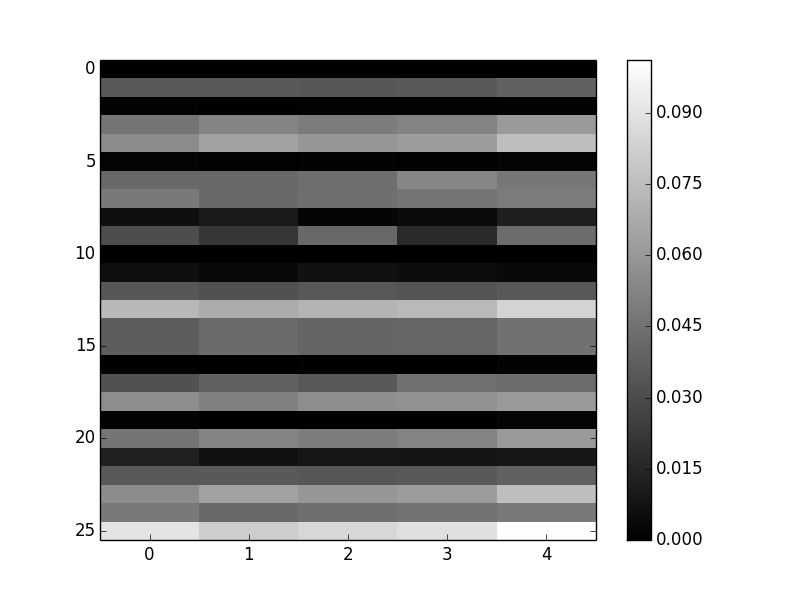
\includegraphics[width=.5\linewidth]{postfreesurfer-nrmse.png}%
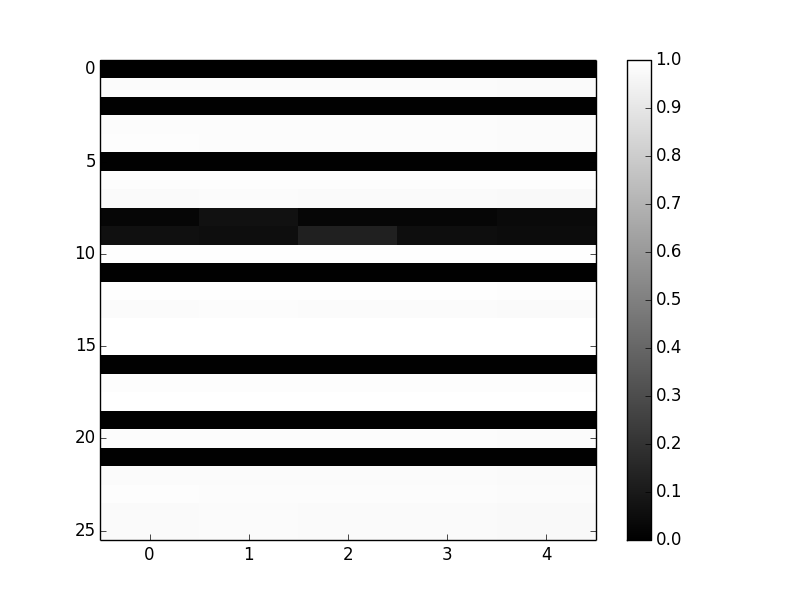
\includegraphics[width=.5\linewidth]{postfreesurfer-dice.png}
\captionof{figure}{PostFreeSurfer metric values}
\caption*{(i) NRMSE (left) (ii)Dice Coefficient (right)}
\label{fig:postfreesurfer_metric_values}
\end{center}

\section{fMRIVolume}\label{sec:fMRI}
\begin{center}
  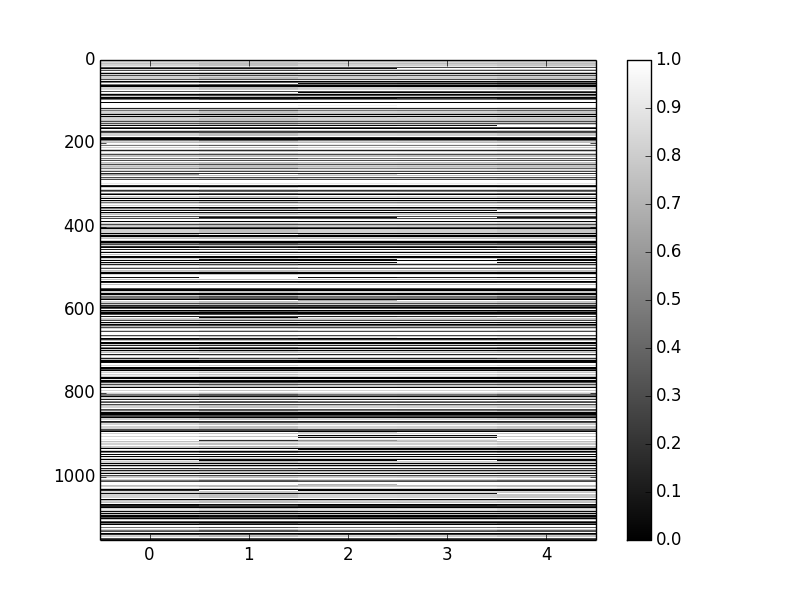
\includegraphics[width=\linewidth]{fmri_DICE.png}
   \captionof{figure}{fMRI Volume Dice}
   \label{fig:fMRI_Dice}
\end{center}

\begin{center}
  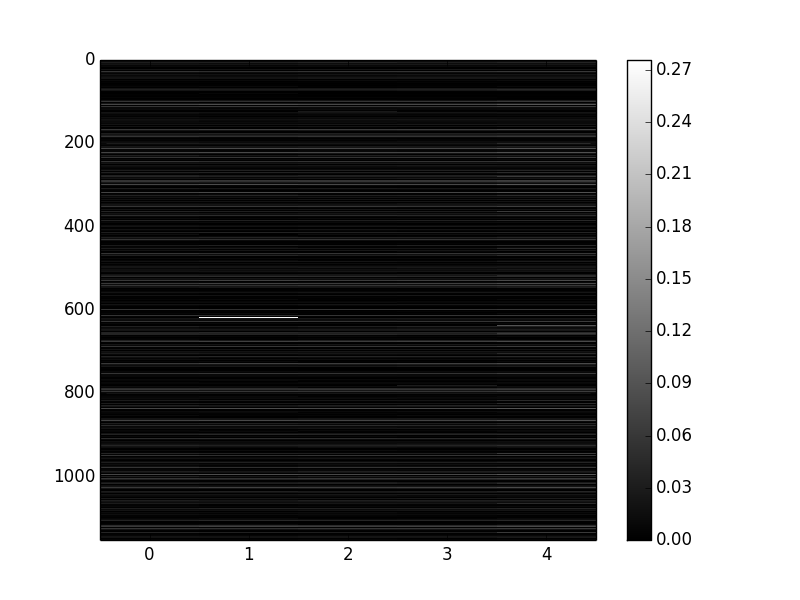
\includegraphics[width=\linewidth]{fmri_NRMSE.png}
   \captionof{figure}{fMRI Volume NRMSE}
   \label{fig:fMRI_NRMSE}
\end{center}
